% This is LLNCS.DOC the documentation file of
% the LaTeX2e class from Springer-Verlag
% for Lecture Notes in Computer Science, version 2.4

\documentclass{llncs}
\usepackage{llncsdoc}

\usepackage{url}

\usepackage{graphicx}
\usepackage{graphics}

\usepackage{pgfplots}
\usepackage[utf8]{inputenc}
\newtheorem{cnj}{Conjecture}

\usepackage{amsmath}
\usepackage[utf8]{inputenc}

%
\begin{document}

\title{Cyber-insurance \& endogenous network formation}

\author{Håvard Råmundal Halse\inst{1}, Jonas Hoemsnes\inst{1} \and Gergely Biczók\inst{2}}

\institute{Dept. of Telematics \\
Norwegian University of Science and Technology \\ \{havahals, jonashoe\}@stud.ntnu.no
\and
Dept. of Telematics \\
Norwegian University of Science and Technology \\ gbiczok@item.ntnu.no}

\maketitle
%

\begin{abstract}
Cyber-insurance is a powerful economic concept that can
help companies in the fight against cybercrime. From the early 80s, several
researchers claimed that cyber-insurance had a bright future, were it
would become a huge economical tool for handling residual cyber-risks.
However, both the European and US cyber-insurance market have failed
to grasp its promising potential. To fully grasp this potential they need
innovative approaches to handle the unique problems of cyber-insurance.
This paper find and characterize network structures with properties that
make them superior as cyber-insurance. And creates several models for
forming these network structures. In every model, new properties that
relate the model to the real-world and real-world insurance products are
added. The results show that insurers can use the insurance premium as
a tool for determining the resulting formation of the network, and if set
to the right level, these superior structures will evolve.
We believe our findings could help the cyber-insurance market evolve, by
giving the insurers a proper tool to better analyze and control formation
of cyber-insurance networks.
\end{abstract}
%
\section{Introduction to cyber-insurance}
Security breaches are increasingly prevalent in the Internet age causing huge financial losses
for companies and their users. When facing security breaches and risk, there are typically four ways to act \cite{bolot:cyber}:
Avoid the risk, retain the risk, self protect and mitigate the risk and transfer the risk

%\begin{enumerate}
%\item Avoid the risk
%\item Retain the risk
%\item Self protect and mitigate the risk
%\item Transfer the risk
%\end{enumerate}
The ICT industry have so far tried to prevent risks with a mixture of options two and three. This has lead to many different techniques and software trying to detect threats and anomalies, to protect the users and infrastructure. Firewalls, intrusion- detection and prevention systems, are some of the solutions. These will reduce the risk, but do not eliminate the risk completely. Although they are all good and needed actions, it is impossible to achieve perfect cyber-security, due to many reasons: Threats are continuously evolving, there will always be accidents and security flaws, attackers have different intentions, network externalities and free-riding in security networks, the lemons-market in security products, misaligned incentives between users and product vendors, and many more. 
This is why we need cyber-insurance, as an fourth option, to handle the residual risk \cite{bolot:cyber2,ranjan:cyber}.

The market for cyber-insurance emerged in the late 80's, when security software companies began collaborating with insurance companies to offer insurance policies together with their security products. From a marketing perspective, adding insurance helped highlighting the supposedly high quality of the security software. Nevertheless, this new product was a comprehensive solution, which dealt with both risk reduction and residual risk \cite{bolot:new}. Continuing into the beginning of the new millennium, several companies started offering standalone cyber-insurance, which sat the frame for the current insurance product. However, as found in the papers \cite{ccost,evolvingcyber,CFCunder} both the US and the european market have not managed to reach its promising potential. Companies are weekly suffering from successful attacks, but most firms still have not acquired cyber-insurance. 
Researchers claim that the main reasons that cyber-insurance is struggling is the three unique problems, information asymmetry, correlated risk and interdependent agents \cite{bohme2010modeling}. 
  \paragraph{Information asymmetry.}
Information asymmetry arises when one side of a transaction or decision has more or better information than the other party. There are two different cases of information asymmetry. The first one is called adverse selection, where one party simply has less information regarding the performance of the transaction. A good example for the cyber-industry, where an insurer has trouble confirming whether your computer/network is "healthy".
The other information asymmetry scenario is called moral hazard. It occurs after the signing of the contract, where one party deliberately takes some action that makes the possibility of loss higher, e.g. choosing not to lock your door. Or in the computer setting, deliberately visiting hostile web-pages, or not using anti-virus software, firewalls or other self-protection software, although you are required to do so. 
      
\paragraph{Correlated risk.}

Another big concern regarding cyber-insurance, is the correlated risk. Among other things, the problem occurs due to the need for standards. Standardization is an important part of the business of computers and computer networks. Generally it enables computers to communicate, install and use different software. A good example is operative systems for personal computers, today we only have a small set of operative systems available, and these systems are standardized, so they can use the same communication channels. The standards generate a lot of the value in the ICT industry, but they also make many threats possible. All systems that use the same standards, create a large number of similar exposure units which could be exploited at the same time. 
Thus create a significant difficulty for the cyber-insurance industry, because when a security breach occurs there is a high probability that it will occur to a large number of people.
 
 \paragraph{Interdependent security.}
Another problem in the ICT industry is interdependent security, meaning that you are not only dependent on your own investment in security, but also on everyone else's. 
Investment in security generates positive externalities, and as public goods, this encourages free riding. The problem is that the reward for a user investing in self-protection depends on the security in the rest of the network. i.e. The expected loss due to a security breach at one agent in the network, is not only dependent on this agent's level of investment in security, but also on the security investment done by adjacent agents, and their adjacent agents and so forth.
  
The cyber-insurance market seem to have a huge potential, but needs some new thinking to fully take advantage of it. We will take a new approach where we focus on finding network structures that will be beneficial for cyber-insurance, and see if it i possible for insurers to force these structures to evolve.


\section{Cyber-insurance network structures}

Like many phenomenons in our society, the cyber-insurance market can be described using graphs. Therefore we will see if there exists any graph structures that would be desirable for a cyber-insurance market.

As a start, the paper \cite{lieberman2005evolutionary} is about evolutionary dynamics and how some structures
can amplify or sustain evolution and drift\footnote{Drift is the opposite of selective evolution, it is when the network/structure evolve and change at random}.
One aspect of cyber-insurance is risk, and knowledge of how, for example, viruses spread in a network and how to use graph structures to prevent both hackers from entering and virus from spreading, is important. Evolutionary dynamics, and the research of how mutant genes spread throughout a population, as described in the paper, is analogous to this issue.
If we can determine some structures where certain nodes are advantageous/disadvantageous, then these structures will have important properties, such as sustaining viruses from spreading.

Another paper, \cite{lieberman2005evolutionary}, shows that mutants inserted into a circulation graph, will have a fixation probability equal to
\begin{equation}  
p_{1}=\frac{(1-\frac{1}{r})}{(1-\frac{1}{r^{N}})}
 \label{eq:fixation} 
\end{equation}
Where $r$ represents the relative fitness of the mutant i.e the agents security level, if it is advantageous it will have a certain chance of fixation, and disadvantageous mutants will have a chance of extinction. A circulation graph is a graph that satisfies these two properties: 
\begin{enumerate}
\item The sum of all edges leaving a vertex is equal for all vertices
\item The sum of all edges entering a vertex is equal for all vertices
\end{enumerate}
A clique is a good example of a circulation graph, and the probability of fixation is as in Eq.(\ref{eq:fixation}).
The fixation probability determines how probable it is that the whole network will eventually be
"infected" by the mutant. Which means that it determines the rate of evolution, which relies on both the size of the
network and the evolution speed. 
If the relative fitness of the nodes is high, then the probability of fixation will be low.
A probability equal to one means that every node in the network will eventually be affected by the mutant.

An essential part of cyber-insurance is as mentioned earlier, for the insurer to be able to calculate the overall risk of the instance to be insured. Since the probability of fixation can be calculated in circulation graphs, if the insurer knows that the instance is part of a circulation graph, it is possible for the insurer to calculate the probability of fixation in that network. 
If we can find graphs with a fixation probability that exceeds Eq.(\ref{eq:fixation}) it is even better, because then the insurer is not only able to calculate the overall probability of fixation, but also to show that the probability of fixation is higher than the one for circulation graphs.

\cite{lieberman2005evolutionary} shows that such graphs exist, and one example is the star topology.
In this topology the fixation probability is as shown in Eq.(\ref{eq:fixation2}), or more generally Eq.(\ref{eq:fixationk}). $K$ is an amplifier parameter, the star-structure has an amplifier $K=2$. The super-star, funnel and metafunnel can all be extendend to arbitrarily large K, thereby guaranteeing the fixation of any advantageous mutant. \cite{lieberman2005evolutionary}.

\begin{equation}p_{2}=\frac{(1-\frac{1}{r^{2}})}{(1-\frac{1}{r^{2N}})} \label{eq:fixation2} \end{equation}.

\begin{equation}
p_{k}=\frac{(1-\frac{1}{r^{k}})}{(1-\frac{1}{r^{kN}})} \label{eq:fixationk}
\end{equation}
 When comparing Eq.(\ref{eq:fixation}) and Eq.(\ref{eq:fixation2}), we see that the selective difference is
 amplified from $r$ to $r^{2}$, i.e. a star acts as an evolutionary amplifier, favoring advantageous
  mutants and inhibiting disadvantageous mutants.

The paper \cite{contagion} present interesting results regarding network formation games. 
The authors set up a game where the nodes benefit from direct links, but these links also expose them to risk. 
Each node gains a payoff of $a$ per link it establishes, but it can establish a maximum of $\delta$ links.
A failure occurs at a node with probability $q$, and propagates on a link with probability $p$. If a node fails, it will receive a negative payoff of $b$, no matter how many links it has established. The characteristics of this game is transferable to how we expect nodes in a cyber-insurance network to interact with eachother. Therefore, the results of the overall payoff change according to different collection of participants. 

The results from the model presented by Blumen et.al. shows a situation where clustered graphs achieve a higher payoff when connected to trusted nodes, compared to when connecting with random nodes. Unlike in anonymous graphs, where nodes connect to each other at random, nodes in these graphs share some information with their neighbors, which is used when deciding whether to form a link or not. 
To further explain these results, they show that there exists a critical point, called \textit{phase transition}, which occurs when nodes have a node degree of $\frac{1}{p}$. 
At this point a node gets a payoff of $\frac{a}{p}$, and to further increase the payoff the node needs to go into a region with significantly higher failure probability. 
Because once each node establishes more than $\frac{1}{p}$ links, the contagious edges will with high probability form a large cluster, which results in a rise in probability of node failure, and reduces the overall welfare.
From this the paper states that when the minimum welfare exceeds 
$(1+f(\delta)*\frac{a}{p})$
we have reached \textit{super-critical payoff}. Otherwise it is called \textit{sub-critical payoff}. 
Further Easley et.al, show that the only possible way of ending up with super critical payoff, is by forming clustered networks consisting of cliques with slightly more than $\frac{1}{p}$ nodes. 
However, if the nodes form an anonymous market, by random linking, they can only get sub-critical payoff. 
In other words, if the nodes can choose who they connect with, and by doing so, create trusted clustered markets, they can achieve a higher payoff by exceeding the critical node degree point. 

\paragraph{From an insurer's point of view.}

 Can the insurer force cyber-insurance networks to evolve into any of these structures, and at the same time separate the nodes into trusted and untrusted environments? 
If so, this could contribute significantly to solving the problems of cyber-insurance. The problems of information asymmetry and interdependent risk is reduced. Because, if the insurer knows the network structure, he can calculate the probabilities of failure and catastrophic events. 

\subsection{Research Question}

Until now, our paper has introduced cyber-insurance, presented related work on the issues regarding cyber-insurance and this chapter has presented the properties of different graph structures and briefly introduced the idea of network formation. 
In this section, we have shown some structures, especially the star and clique, which could generate benefit for both the insurer and customers in a cyber-insurance market. 
We will combine the knowledge of these structures and network formation games to investigate networks consisting of nodes, insured or not, wanting to increase their payoff by establishing links with eachother. Is it possible for the insurer to force these networks to evolve endogenously into these structures?
We will focus on how the insurer can determine the resulting formation by adjusting the parameter he can control, i.e. the insurance cost. We know that if the insurance premium is too high, no one will buy it. On the other hand, if it is too low, everyone would benefit from having insurance, and insured nodes will make risky decisions, such as connecting to risky nodes. We will try to determine whether it is possible to find the intersections, where the desired structures will evolve, and both the insurer and their customers will benefit from this.


\section{Modeling Cyber-insurance}


\section{Models}
There are many examples of nodes that need to establish connections with eachother.
For example, when a firm is outsourcing tasks, cooperating or depending on other
firms in some way. Such scenarios could be modeled, as networks where the nodes
represents the firms and the links between them are their dependencies. However,
the link between nodes involves some risks, such as: will the company deliver at the
reported time, to the reported costs, what happens if it fails to deliver, what if the
company goes bankrupt etc. To handle these risks, we need cyber-insurance.


When deciding whether or not to establish a link to a node, the payoff has to be
higher in the balance between the expected earnings and the risk of the other party
failing to complete the transaction. From the insurer’s point of view, a problem
with cyber-insurance is to define and calculate risk, because the network structure is
undefined. If an insurer were able to predict the network structure, the calculations
of overall risk would be realizable. The situation could be even better if the insurer
could force a chosen robust network structure to evolve, hence, ensuring a higher
total payoff for the network. Examples of such structures are scale-free networks,
stars and cliques, as described in the graph theory chapter. In summary, scale-free
networks have proven to be very robust against random attacks. Star topologies, or
star-like topologies, have a fixation probability that exceeds the fixation probability
of circulation graphs. Star structures also have a desirable property of minimizing the
average path length, i.e. minimizing the cost spent on establishing links. Finally, the
clique has a nice property of being able to achieve super-critical payoff, as showed in
[Blu11]--FIX. In our thesis we want to focus on the clique and star/star-like structures for
the following reasons: Both have been identified to have calculable fixation probability
and the possibility of amplifying or suppressing selection and drift. This is favorable,
because if the insurer is able to ensure that the nodes have a certain security level,
particularly the center node, one can prevent viruses from spreading to other nodes.

In our models a node is an agent who is either insured or not, and the nodes’ goal is to maximize its payoff, by establishing links with other nodes. Our goal for the models is to find out if and how an insurer can force these cyber-insurance networks to evolve into the desirable structures mentioned in previous sections.
The different parameters used to modes the formation games are denoted as follows: The insurance premium is $I_{l}$, the expected risk cost is represented by $r$. $\beta$ represents the benefit of establishing a link. Additionally is the process of establishing links a bidirectional decision between the nodes. 
 

\section{Model 3: Including maximum node degree and bonus}
Our first model reflects a normal phenomenon occurring in networks. In real world networks, such as in the manufacturing industry, software development firms and many other types of business, in some scenarios a product can usually not be completed without outsourcing some of the work needed. For the manufacturer, it could be beneficial to buy certain parts from others instead of producing them on his own. A software product might need the combined knowledge from different firms. Thus the firm that outsources tasks is dependent on the other firms, and will not reach its goal before the other firms deliver their contribution. When the product is finished the company gets paid.
To model this scenario we introduce a maximum node degree, $m$, per node, which represents the number of partners needed to complete a task. Additionally a bonus $\gamma$ represents the payoff a node receives when $m$ links are established. 

  
When establishing a link between two insured nodes, the payoff the nodes will receive is as described in Eq.(\ref{eq:itoi}).
Let $U_{i}$ denote the payoff of a node with degree i, and let $U_{i+1}$ be the payoff
a node will receive if it establishes a new link.
\begin{equation}
    U_{i+1}= 
\begin{cases}
    \beta - I_{l},& \text{if } i = 0\\
    U_{i}+\beta -I_{l},& \text{if }  i>0\\
    U_{i}+\beta -I_{l}+\gamma,& \text{if } i=m-1
    
\end{cases}
\label{eq:itoi}
\end{equation}


\subsection{Analysis}
For nodes to connect to each other, the change in payoff has to be positive: $U_{i+1} > U_{i}$. However, we also need to consider the bonus received when reaching the maximum node degree, $m$. 
To model this, we add the possible bonus divided on the number of links required to reach the bonus($\frac{\gamma}{m-i}$) in the decision process every time a node is considering to establish a link. 
In this way the model will change from the earlier models, because now the nodes have more incentive to connect to other nodes, and for every step closer to the goal, the nodes are more willing to accept risk than before. For example, an insured node is more likely to accept a risky link when it only needs one more link to reach the goal, compared to when it need several more links to reach the goal.

 The model now introduces a risk factor, because it is not certain that the nodes will obtain enough links, and if not, they will not receive their bonus, and they are stuck with their already established connections. 

To analyze this model, let us take a closer look at the four different scenarios of the game. When establishing a link between two insured nodes, the payoff the nodes will receive is as described in Eq.(\ref{eq:itoi}).
\begin{equation}
    U_{i+1}= 
\begin{cases}
    \beta - I_{l},& \text{if } i = 0\\
    U_{i}+\beta -I_{l},& \text{if }  i>0\\
    U_{i}+\beta -I_{l}+\gamma,& \text{if } i=m-1
    
\end{cases}
\label{eq:itoi}
\end{equation}
As described earlier we need to include the possibility of reaching the goal in the decision, and thus for insured nodes to connect to each other, Eq.(\ref{eq:itoi2}) has to hold.
\begin{eqnarray}
U_{i}+\beta-I_{l}+\frac{\gamma}{m-i}&>U_{i} \nonumber \\ 
\beta-I_{l}+\frac{\gamma}{m-i}&>0 \nonumber \\ 
\llap{$\rightarrow$\hspace{50pt}} \beta+\frac{\gamma}{m-i}&>I_{l} 
\label{eq:itoi2}
\end{eqnarray}

The payoff an insured node receives when connecting to a non-insured node is as follows:
\begin{equation}
    U_{i+1}= 
\begin{cases}
    \beta  - I_{l} -r,& \text{if } i = 0\\
    U_{i}+\beta -I_{l}-r,& \text{if }  i>0\\
    U_{i}+\beta -I_{l}-r+\gamma,& \text{if } i=m-1
\end{cases}
\label{eq:itonoti}
\end{equation}
To establish a connection from an insured node to a non-insured one, the following has to hold:
\begin{eqnarray}
U_{i}+\beta-I_{l}-r+\frac{\gamma}{m-i}&>U_{i} \nonumber \\ 
\beta-I_{l}-r+\frac{\gamma}{m-i}&>0 \nonumber \\ 
\llap{$\rightarrow$\hspace{50pt}} \beta+\frac{\gamma}{m-i}-r&>I_{l} 
\end{eqnarray}

When a non-insured node connects to another non-insured node, this is the payoff they both will receive:
\begin{equation}
    U_{i+1}= 
\begin{cases}
     \beta -r,& \text{if } i = 0\\
    U_{i}+\beta -r,& \text{if }  i>0\\
    U_{i}+\beta -r +\gamma,& \text{if } i=m-1
\end{cases}
\label{eq:noitonoti}
\end{equation}
To establish the connection, the following equation has to hold:
\begin{eqnarray}
U_{i}+\beta-r+\frac{\gamma}{m-i}&>U_{i} \nonumber \\ 
\beta-r+\frac{\gamma}{m-i}&>0 \nonumber \\ 
\llap{$\rightarrow$\hspace{50pt}} \beta+\frac{\gamma}{m-i}&>r
\end{eqnarray}
In the case of a non-insured node wanting to establish a link with an insured node, the payoff is a strictly increasing function, see Eq.(\ref{eq:noitoti}), and thus a non-insured node will always connect to an insured node if possible.
\begin{equation}
    U_{i+1}= 
\begin{cases}
    \beta,& \text{if } i = 0\\
    U_{i}+\beta,& \text{if }  i>0\\
    U_{i}+\beta +\gamma,& \text{if } i=m-1
\end{cases}
\label{eq:noitoti}
\end{equation}

\subsection{Result and findings}

If we want a clique of only insured nodes, we have to ensure that insured nodes connect to each other, and that they do not establish connections to non-insured nodes.
We know that an insured node would want to connect to another insured node if  Eq.(\ref{eq:itoi2}) is satisfied. 
In the equation we see that the expected bonus per established link is increasing. Thus, if an insured node of degree zero is willing to connect to another insured node, then every insured node with a degree higher than zero would also like to connect to another insured node. To ensure that insured nodes connect to eachother this equation has to hold:
\begin{equation}
\beta+\frac{\gamma}{m}>I_{l}
\label{eq:conditionitoi}
\end{equation}
We also want to ensure that insured nodes never establish links with non-insured nodes, from Eq.\ref{eq:itonoti} we see that this has to hold:
\begin{equation}
\beta+\frac{\gamma}{m-i}-r < I_{l}
\label{eq:conditionitonoti}
\end{equation}
This can be simplified, if one can ensure that the most risk willing insured node, i.e. the node with degree $m-1$, does not establish links with non-insured nodes. Then we know that no insured node with degree less than $m-1$ will establish links with non-insured nodes. From this we get equation Eq.(\ref{eq:condition-i-to-noti}).

\begin{eqnarray}
\beta+\frac{\gamma}{m-(m-1)}-r&<I_{l} \nonumber\\
\llap{$\rightarrow$\hspace{50pt}} \beta+\gamma-r&<I_{l}
\label{eq:condition-i-to-noti}
\end{eqnarray}

To summarize, Eq.(\ref{eq:conditionitoi}) and Eq.(\ref{eq:condition-i-to-noti}) give the final limitation on the link insurance cost, Eq.(\ref{eq:final-insurance-clique-condition}). If this equation is satisfied, the resulting network will contain a clique of only insured nodes.
\begin{equation}
\beta+\gamma-r<I_{l}<\beta+\frac{\gamma}{m}
\label{eq:final-insurance-clique-condition}
\end{equation}
For this to even be possible, $\beta+\gamma-r<\beta+\frac{\gamma}{m}$, i.e. Eq.(\ref{eq:noinsuredcliqueconditon}) has to hold. This equation reflects that as the risk to bonus ratio gets smaller, it gets more and more difficult to ensure a clique of only insured nodes. When the risk to bonus ratio is less than $1-\frac{1}{m}$, a clique will never occur. The equation shows that a node would be more and more willing to take a risk, as the reward of doing so increases.
\begin{eqnarray}
\gamma-r &<\frac{\gamma}{m}\nonumber \\
1-\frac{r}{\gamma}&<\frac{1}{m} \nonumber \\
\llap{$\rightarrow$\hspace{50pt}}1-\frac{1}{m}&<\frac{r}{\gamma}
\label{eq:noinsuredcliqueconditon}
\end{eqnarray}

It is also useful to know when non-insured nodes connect to each other. This happens when Eq.(\ref{eq:noitonoti}) is satisfied. This equation is dependent on the node degree, and thus for the first link to be established from a non-insured node, the expected payoff has to be higher than the risk($\beta+\frac{\gamma}{m}>r$). If the risk is too high, then the non-insured node must establish links with insured nodes before it coulb be willing to establish risky links.

With these findings, an insurer can determine the outcome of the network formation game by adjusting the insurance cost parameter.
If he wants a clique of only insured nodes Eq.(\ref{eq:final-insurance-clique-condition}) has to
hold. However, it is easy to relax the condition, so that insured nodes only connect to, $j=1,2,3..m$ non-insured nodes.
   This is done by changing Eq.(\ref{eq:condition-i-to-noti}) to $\beta+\frac{\gamma}{m-(m-j)}-r<I_{l}$, which
    gives us Eq.(\ref{eq:lower-boundary-link-insurance-cost}).
An interesting result in this model is that due to the risk willingness among the nodes, the lower boundary, to ensure separation of insured and non-insured nodes, of the link insurance cost is higher compared to the one found in model 2. 

\paragraph{Consequences of not reaching the required number of edges.} When a node establishes a link, it does not know whether it will reach the maximum node degree, unless the current node degree is $m-1$. Hence the node might end up not reaching the desired goal. This can happen if there is not enough nodes willing to establish links. Consequently, nodes who do not reach their goal could end up with a payoff less than $U_{0}$. 

\begin{equation} 
\beta+\frac{\gamma}{j}-r<I_{l}
\label{eq:lower-boundary-link-insurance-cost}
\end{equation} 



\paragraph{Efficiency and Stability.}

In this model, the incentive for establishing links is increased compared to model 2. Thus, to maintain a stable network with two cliques the cost of link establishment has to be increased. This increased incentive may result in a higher price of stability, but if every node has received its bonus, then the price of anarchy is 1. The price of anarchy is dependent on the number of nodes in both cliques, and whether its enough nodes for everyone to reach their maximum degree or not. 
If there are nodes that have not reached their maximum degree in both cliques, then the resulting network is not necessarily the most efficient, and we could be missing a potential payoff due to the cost constraint. 

By introducing the maximum degree $m$ we are limiting the problem of price of anarchy, because as long as $m$ is less than the number of insured and number of non-insured nodes, there will be less links established compared to model 2, and overall fewer possible links between insured and non-insured. However, the bonus the nodes receive will contribute to inefficiency, because when nodes do not reach their maximum degree, the potential payoff that could be generated by allowing insured and non-insured nodes to connect, is greater than in model 2.


\subsection{Simulation of the results}
For the first simulation the parameters are set to the following: $\beta=0.9, I_{l}=0.7, r=0.5, \gamma=0.2 \text{ and }m=4$, in order to satisfy condition Eq.(\ref{eq:final-insurance-clique-condition}), and enable all nodes to reach their maximum degree.  

\begin{figure}[h]
\centering
  \includegraphics[width=0.7\linewidth]{../Figures/BonusGameInsuredClique.png}
  \caption{\label{fig:bonusoptimal} Two cliques, one consisting of insured agents the other consists of non-insured. All nodes have reached their goal. }
\end{figure}
As we see in Figure \ref{fig:bonusoptimal}, the results were as expected, the cost of insuring a link satisfied the conditions found earlier, and thus the result was two cliques, one consisting of only insured nodes and the other of non-insured nodes.
An interesting observation is that $\beta$ and $r$ is the same as in model 2, but to ensure that only insured nodes connect to eachother, the link insurance cost had to be higher. This is to compensate for the risk the nodes now are willing to take. The price of anarchy in this scenario is 1, i.e. the socially optimal outcome. 

In the second simulation we set the parameter $m=5$, and kept the other variables unchanged. The resulting network was as expected the same as in the last simulation, but since the nodes did not reach their maximum degree, the price of anarchy is less than one. The price of anarchy can be seen in Eq.(\ref{eq:model-bonus-poa}).
\begin{eqnarray}
PoA&=\frac{\text{Sum of payoffs}}{\text{Sum of Socially optimal payoffs}}  \nonumber \\
PoA&=\frac{5\times 4\times (0.9-0.7)+5\times 4\times(0.9-0.5)}{5\times 4\times (0.9-0.7)+5\times 4\times(0.9-0.5)+5\times (2\times 0.9-0.7-0.5 + 2 \times 0.2)}\nonumber \\
PoA&=\frac{12}{17}
\label{eq:model-bonus-poa}
\end{eqnarray}

When we changed the link insurance cost, and set it to the same value as in model 2, $I_{l}=0.5$, the resulting networks change. Now we found that the insured nodes are willing to establish risky links to reach their maximum degree. Some of the resulting networks can be seen in Figure \ref{fig:bonusviolating}.
In figure \ref{fig:bonusvolating:a} the price of anarchy is $0.95$, and in figure \ref{fig:bonusvolating:b} the price of anarchy is $1$, i.e. it has reached the socially optimal outcome.

\begin{figure}
  \centering
  \includegraphics[width=0.55\linewidth]{../Figures/BonusGameViolating.png}
  \caption{\label{fig:bonusvolating:a} One non-insured node has connected to two insured nodes.}
\end{figure}
\quad
\begin{figure}
  \centering
  \includegraphics[width=0.55\linewidth]{../Figures/BonusGameViolatingOptimal.png}
  \caption{\label{fig:bonusvolating:b}Every non-insured node is connected to one insured node, this is the optimal outcome with these parameters.}
\end{figure}
  
 [Two possible outcomes when insured nodes are willing to take the risk of connecting to non-insured nodes, to receive their bonus.]{\label{fig:bonusviolating} Two possible outcomes when insured nodes are willing to take the risk of connecting to non-insured nodes, to receive their bonus. Figure $a$ shows a scenario where one non-insured node has connected to more than one insured node, thus not a socially optimal outcome. Figure $b$ shows the optimal outcome. }



\section{Model 4: Including bulk insurance discount}

Insurance companies often give a quantum discount when a customer purchases multiple products. From convenience stores, we are used to the slogan "buy one get one for free", and insurers tend to follow the same marketing strategy. It seems to be common for insurance companies to offer discount to their customers if the customers choose to combine some or all of their insurances with them. Several insurance companies in Norway, e.g. Sparebank 1 offers customers up to 25 $\%$ discount according to the following rules \cite{sparebank1}. 

\begin{itemize}

\item 10$\%$ discount if the person has signed three different insurances
\item 15$\%$ discount if the person has signed four different insurances
\item 20$\%$ discount if the person has signed five or more different insurances
\item Plus additional 5$\%$ discount if the person is a customer of the bank. 

\end{itemize}

The insurance offered is intended for the individual market and includes among other things: travel insurance, household insurance, car insurance, house insurance, insurance of valuable items and yacht insurance.

Inspired by these kinds of discounts on insurance products, we would like to introduce a discount rate dependent on the degree of the node. In a real-world scenario where nodes have an option of acquiring insurance or not, this will make it more attractive for nodes with high degree to acquire insurance, and the discount could act as an incentive for other nodes to also acquire insurance. Therefore, this seems like a reasonable model to include. Since, if you have many links, you will pay less per link compared to a node having fewer links.

How insurance companies choose to formulate their discount rate might vary. One solution might be to follow a strict 5$\%$ discount per new connection, similar to the one from Sparebank 1, or let the discount follow a power law, or a log-function etc. We choose to follow a discount rule which directly reflects the node's degree.
\subsection{Analysis}
The price for adding a new link follows the equation:
\begin{equation}
\frac{I_{l}}{i+1}
\label{eq:discount0}
\end{equation}
Here, $i$ is the node's current degree. This means that the more links a node establishes the cheaper the link insurance will be. 

\subsubsection{Discount and Bonus model}
We also need to apply the discount to model 3. Still, the only scenarios that has changed in this model is the ones where insured nodes connects to other insured nodes or when insured nodes connects to non-insured nodes.

When insured nodes are considering to establish links with eachother, their payoff functions are as shown in Eq.(\ref{eq:discount1}).  
\begin{equation}
    U_{i+1}= 
\begin{cases}
    \beta - I_{l},& \text{if } i = 0\\
    U_{i}+\beta -\frac{I_{l}}{i+1},& \text{if }  i>0\\
    U_{i}+\beta -\frac{I_{l}}{i+1}+\gamma,& \text{if } i=m-1
\end{cases}
\label{eq:discount1}
\end{equation}
For insured nodes to connect to eachother Eq.(\ref{eq:model4-bonus-i-to-i}) has to hold.

\begin{eqnarray}
U_{i}+\beta-\frac{I_{l}}{i+1}+\frac{\gamma}{m-i}&>U_{i} \nonumber \\ 
\beta-\frac{I_{l}}{i+1}+\frac{\gamma}{m-i}&>0 \nonumber \\ 
\llap{$\rightarrow$\hspace{50pt}}\beta +\frac{\gamma}{m-i}&>\frac{I_{l}}{i+1}
\label{eq:model4-bonus-i-to-i}
\end{eqnarray}

When insured nodes are considering to connect to non-insured nodes, their payoff functions are as shown in Eq. (\ref{eq:model4-bonus-i-to-ni}).
\begin{equation}
U_{i+1}= 
\begin{cases}
    \beta - I_{l}-r,& \text{if } i = 0\\
    U_{i}+\beta -\frac{I_{l}}{i+1}-r,& \text{if }  i>0\\
    U_{i}+\beta -\frac{I_{l}}{i+1}-r+\gamma,& \text{if } i=m-1
\end{cases}
\label{eq:model4-bonus-i-to-ni}
\end{equation}
For this to happen Eq.(\ref{eq:model4-bonus-i-to-ni-final}) has to hold.

\begin{eqnarray}
U_{i}+\beta-\frac{I_{l}}{i+1}+\frac{\gamma}{m-i}-r&>U_{i} \nonumber \\ 
\llap{$\rightarrow$\hspace{50pt}}\beta+\frac{\gamma}{m-i}&>r+\frac{I_{l}}{i+1}
\label{eq:model4-bonus-i-to-ni-final}
\end{eqnarray}

\subsection{Result and findings}
We analyze the same scenario as in the other models, namely a clique of only insured nodes. The first step is to guarantee that insured nodes connect to eachother. To ensure that this happens, we need to find the condition for the lowest expected increase in payoff, i.e. at node degree zero. If nodes are willing to establish links at this point, then they will also be willing at all degrees higher than zero.
At degree zero there is no discount on the insurance link cost, and thus if Eq.(\ref{eq:conditionitoi}) from model 3 holds, insured nodes will connect to other insured nodes.

The condition for guaranteeing that insured nodes do not connect to non-insured nodes has changed, we know that if an insured node does not want to establish a link with a non-insured node at degree $m-1$, then neither will any insured node with degree lower than $m-1$ do so. From this we find the condition in Eq.(\ref{eq:model4-bonus-i-not-ni})
\begin{eqnarray}
U_{i}+\beta-\frac{I_{l}}{m}+\frac{\gamma}{m-(m-1)}-r&<U_{i} \nonumber \\ 
\beta+\gamma-r&<\frac{I_{l}}{m}\nonumber \\ 
\llap{$\rightarrow$\hspace{50pt}}m(\beta +\gamma-r)&<I_{l}\nonumber
\label{eq:model4-bonus-i-not-ni}
\end{eqnarray}
This is a very strong condition, because the only way this can happen is if $\beta+\gamma-r<\frac{1}{m}$.  This shows us that when the incentives for establishing links increase, it gets more and more difficult for the insurer to guarantee a clique of only insured nodes. 
The final condition for ensuring a clique of only insured nodes is shown in Eq.(\ref{eq:model4-final-condition-insured-clique}).

\begin{equation}
m(\beta +\gamma-r)<I_{l}<\beta+\frac{\gamma}{m}
\label{eq:model4-final-condition-insured-clique}
\end{equation}

The quantum discount results in an overall higher payoff for the insured nodes, since the cost of insuring a new link becomes cheaper. This means that the insured nodes will have a higher incentive to create links, making it harder for the insurer to separate insured and non-insured nodes.

We see that the problem of separating the two node types have increased compared to model 3, meaning that if we have a network where the insurer has managed to separate them, the price of anarchy is also higher compared to a similar scenario in model 3. 





\section{Model 5: Network externalities}
In the earlier models, the experienced network effects arose only from a node's neighbours. I.e. when a node established a connection the change in utility were only dependent on fixed variables, and not dependent on the rest of the network. In many real world scenarios it is more realistic that a node will be strongly affected by the indirect connections to other nodes. Social relationships between nodes are good examples of such networks, where each person offer benefits in terms of favors, information etc. 

We apply the results from the paper from Jackson and Wolinsky \cite{jackson1996strategic} and use a network formation game found in \cite{jackson2005survey} to study indirect network effects in our model. 

The benefits a player receives in this game are calculated as follows: In addition to the benefit from the direct connection, a node will also benefit from "friends of the friend", and "friends of the friends of the friend" etc. This is achieved by letting the payoff be calculated relative to the distance between the nodes. $\beta$ now depends on the minimum number of hops to the node, e.g. the benefit of a direct connection is $\beta$, the benefit of a friend of a friend is $\beta^2$ etc. We want the benefit to decrease with distance, therefore we need the limitation: $0<\beta<1$. 
\begin{figure}[h]
\centering
  \includegraphics[width=0.3\linewidth]{../Figures/connectionGame.png}
  \caption{\label{fig:connectionGame} Four nodes interconnected with each other.}
\end{figure}
\paragraph{Example:}Let us consider the network shown in \ref{fig:connectionGame}. Node 1 and node 4 in the network will receive a benefit of $\beta+\beta^{2}+\beta^{3}$ by being connected with nodes 2 and 3. $\beta^{2}+\beta^{3}$ represents the indirect benefits from nodes 3 and 4. Nodes 2 and 3 receive a benefit of $\beta+\beta+\beta^{2}$. For this network to make sense, it is important to also include some cost of having direct connections, or else the rational thing would be to establish a link with everyone. This is done as in earlier models, every node pays a cost for direct connections, but no cost for indirect connections. Thus the total payoff for a node is:

\begin{equation}
\sum_{j\neq i}^{} \beta_{ij}^{d(ij)} - \sum_{j:ij\in g}^{} {c}_{ij}, 
\label{eq:connecetionGame}
\end{equation}

Where $d(ij)$ represents the shortest path between node $i $ and node $j $, and ${c}_{ij}$ represents node i's cost of establishing a link between the two nodes. To simplify the model we choose a symmetric connection process where $\beta$ and $c$ is set to a fixed global value. 

In the paper \cite{jackson1996strategic}, the authors analyze the networks with two different approaches, one with focus on efficiency and the other on stability.  The optimal network is of course both efficient and stable, but as we shall see there are some conflicts between efficiency and stability. Matthew, et.al. showed that an efficient network is:
\begin{enumerate}
\item \textit{a complete graph $g^N$ if $c<\beta - \beta^2$,}
\item \textit{a star encompassing every node if $\beta - \beta^2 < c < \beta + \frac{(N-2)}{2}\beta^2$,}
\item \textit{an empty network (no links) if $\beta + \frac{(N-2)}{2}\beta^2 < c$.}
\end{enumerate}

The most efficient structure is a star structure which encompasses every node. A star structure has the characteristics of minimizing the average path length and uses the minimum number of links ($N-1$) required for including every node. 
This structure provides the highest overall payoff for the network, but this network is not necessarily stable.

When analyzing the stability of the network, by using the definition of pairwise stability, Jackson and Wolinsky found four different stability conditions:

\begin{enumerate}
\item \textit{a pairwise stable network consists of at most one (non-empty) component,}
\item \textit{if $c<\beta - \beta^2$, the unique pairwise stable network will be a complete graph $g^N$, }
\item \textit{if $\beta - \beta^2 <c < \beta $, a star encompassing every node will be pairwise stable, although not necessarily the unique pairwise stable graph,}
\item \textit{if $\beta < c$, any pairwise stable network which is nonempty is such that each player has at least two links and is thus inefficient. }
\end{enumerate}
We see that stability condition 2 is the same as efficiency condition 1, and therefore if this condition is fulfilled, the network is both stable and efficient. 
Condition 3 shows us why the efficient star network is not necessarily stable. If $\beta \leq c <   \beta + \frac{(N-2)}{2}\beta^2$ then the efficient network will be a star, but it is not stable.

It should be noticed that it is more beneficial for a node to operate as a leaf node compared to being a center node, due to the cost of direct connections. In a star structure, a leaf node will only have to pay the cost of the link to the center node, and will benefit indirectly for each node connected to the center node. The center node will benefit from each new connection, but, the payoff will only be $\beta - c$ for each connection. 

\subsection{Insurance and connection game}
The findings about efficiency and stability are very useful for our model, because if one has knowledge of the different variables it is possible to determine how the network will evolve. Additionally, if you are able to control the variables, you can actually determine the resulting network structure.
From the referenced papers, we know that different boundaries on the link cost exists, and how the resulting stable and efficient network will be.
Our earlier models show that the cost of establishing a link is the insurance cost and/or the risk cost. From this we can show that if $\beta - \beta^2 <I_{l}<\beta \text{ and } r>\beta$, a star with only insured nodes, and no connections between non-insured nodes, is both a stable and an efficient network. If $\beta - \beta^2 <I_{l}+r<\beta \text{ and } \beta - \beta^2<I_{l} \text{ and } \beta - \beta^2<r $, the stable and efficient network is a star consisting of both insured and non-insured nodes. If $I_{l}<\beta-\beta^2$ all insured nodes will connect to every other insured node, and if $r<\beta-\beta^2$ all non-insured nodes will connect to every other non-insured node.
In addition if $r+I_{l}<\beta-\beta^2$ the resulting network will be a clique of both insured and non-insured nodes.
The insurer can thus determine the formation of the network by adjusting the cost parameters. 

\subsection{Homogeneous symmetric connection game}
From this point on, the game we will consider is a homogeneous network setting, where every node is considered to be insured.
This is done because it will simplify an otherwise very complex model. We are analyzing the resulting network structure, which is easier when only considering one homogeneous cost for every node.
Let us look at an example, where the parameters are set to: $\beta=0.9, I_{l}=0.5$. The resulting network from a simulation is shown in Figure \ref{fig:stablestar}.



\begin{figure}[h]
\centering
  \includegraphics[width=0.5\linewidth]{../Figures/stability/Unefficientbutstablestar.png}
  \caption{\label{fig:stablestar} The resulting network after a simulation with the parameters $\beta=0.9, I_{l}=0.5$.}
\end{figure}
As we see this is not an efficient star, but the network is stable. The efficient network would be to delete the link $4,6$ and adding the link $1,6$. But since we only consider one link at a time this can not be done. To show this let $U_{i}$ denote the payoff of node $i$, the payoffs of the nodes are as described in Eq.(\ref{eq:payoffstablestar}).
\begin{eqnarray}
U_{1}=4\beta+\beta^2-4c\nonumber\\
U_{2}=U_{3}=U_{5}=\beta+3\beta^2+\beta^3-c\nonumber\\
U_{4}=2\beta+3\beta^2-2c\nonumber\\
U_{6}=\beta+\beta^2+3\beta^3-c
\label{eq:payoffstablestar}
\end{eqnarray}
Node $6$ would benefit from adding the link $1,6$, but node 1 is not willing to do so, because then it must pay an extra cost, and since $\beta^2>\beta-c$, the network is stable, but not efficient. 

From this we see that, even when the most efficient and stable network is a star, we can not guarantee that the network formation game will end up in a star. This is because we only consider one link at a time, and not the whole network. 

\paragraph{A star is not possible with high \textit{n}.}
In the paper \cite{jackson2005survey} the authors came up with the following proposition:
Consider the symmetric connections model in the case where $\beta-\beta^2<c<\beta$. As the number of nodes grows, the probability that a stable state (under the process where each link has an equal probability of being identified) is reached with the efficient network structure of a star goes to zero. But if a network reaches the efficient star structure, it is also pairwise stable, and will remain a star. 
We confirmed this when running multiple simulations. When we used few nodes the resulting network often became a star, but as the number of nodes increased the network rarely became a star. 

However, the structure of the networks that evolve is very similar to a scale-free network. There are many nodes with low node degree, and few with a high node degree.
One example of this is shown in Figure \ref{fig:stablescalefree}. There are only ten nodes, but the network has the properties of a scale-free network. Two nodes have a degree of 4, and the rest have a degree of one or two.
\begin{figure}[h]
\centering
  \includegraphics[width=0.6\linewidth]{../Figures/stability/Unefficientbutstabletwo.png}
  \caption{\label{fig:stablescalefree} The resulting network after a simulation with the parameters described earlier and 10 nodes.}
\end{figure}
\paragraph{Bulk insurance.}
As noted before it is not preferable to be the center node, due to the cost of all the direct links. In a model with bulk insurance discount, the extra cost for the center node would decrease significantly. This could be used to increase the probability of reaching a star formation. 

Using the discount formula from the previous model, we end up with Eq.(\ref{eq:discountstar}) to achieve an efficient and stable star topology. $i$ represents the node degree.
\begin{equation}
\beta-\beta^2<\frac{i_{l}}{i+1}< \beta
\label{eq:discountstar}
\end{equation}
An interesting property of the discount model is that the conditions for efficient and stable networks will change. Because
when the node degree increases, the insurance cost might reach the critical degree $g$, and the best strategy for a node with degree $g$ or higher, is to connect to every node, as shown in Eq.(\ref{eq:criticaldiscount}). The critical degree occurs when a node's optimal strategy changes from relaying on indirect connections to connecting to every node. 
\begin{equation}
\frac{I_{l}}{g}<\beta-\beta^2
\label{eq:criticaldiscount}
\end{equation}
This is possible when $g<n$, where $n$ represents the number of nodes in the network.
The stability condition has changed for a node with a critical degree. The stable and efficient condition for this node is, as shown earlier, to have a direct connection to every other node. Thus if we have a star topology, both the leaf nodes and the center node are stable, and the center node has been compensated for its role in the network.

Since the networks formed are similar to scale-free networks, we can calculate the probability of a node having degree $g$, see Eq.(\ref{eq:probabilitydegree}). $\gamma$ is the power law parameter, as described in Chapter 4.
\begin{equation}
P(g)=g^{-\gamma}
\label{eq:probabilitydegree}
\end{equation}
When a node $i$ reaches the critical degree $g$ its optimal strategy is to connect to every node, since the payoff generated from direct connections is larger than any indirect connection. In general, nodes prefer to connect to nodes with high connectivity\footnote{A node with high degree implies a node with high connectivity.}, and will thus prefer to connect to this node compared to nodes with a degree lower than $g$. In this way, nodes will connect to the node who has a degree greater than or equal to $g$, and remove the links to their low-degree nodes which they can instead reach through the node with high connectivity.

Let us consider a case with $n$ nodes, and two of these nodes, $i$ and $j$, have an equal degree larger than $g$. The rest of the nodes have a degree of one or zero. If there exists a node with degree zero, it would prefer to be connected to $i$ or $j$, and so will $i$ and $j$, so this will eventually happen.
If a node connected to $i$ is considering connecting to $j$, or vice versa, it will do so because $j$ can offer a higher connectivity than $i$. Now $j$ has a higher degree than $i$, and thus every node would prefer to connect to $j$ over $i$. This will eventually result in a star formation, with $j$ as the center node.
From this we get the conjectures:
\begin{cnj}
If the critical degree ratio is low, i.e. the ratio between critical degree and number of nodes in the network, the resulting network will with high probability be a clique.
\label{prop:clique}
\end{cnj} 

\begin{cnj}
If the critical degree ratio is at a medium level, the resulting network will with high probability be a star. 
\label{prop:star}
\end{cnj}

\begin{cnj}
If the critical degree ratio is high, the resulting network will with high probability be a star-like/scale-free structure. 
\label{prop:scale-free}
\end{cnj}

A numerical example of the boundaries between the different structures, we found from our simulation (described in the next section) with 20 nodes is the following: 
As seen in Figure \ref{fig:PlotStar} a critical degree of 1-5 applies to conjecture \ref{prop:clique}, 6-12 applies to conjecture \ref{prop:star} and 13-20 applies to conjecture \ref{prop:scale-free}. 

\subsubsection{Results and findings}

To prove the conjectures above, we created a simulator. The rules of the simulator are as following:
Every round of the game,two random nodes, not neighbors, are selected, and asked if they would want to establish a link. The link establishment is a symmetric decision, i.e. the link is established if it result in an increased payoff for both nodes. If the link is added, we check if either of the nodes would prefer to delete some of their already existing links, this decision is asymmetric. A link will be deleted if the node will achieve a higher payoff without it. Then we ask the rest of the nodes if they would like to delete any links. This procedure is repeated as long as it is possible to add new links. 
The payoff function of each node is as described earlier (see Eq.(\ref{eq:connecetionGame})), except that the cost is now dependent on the degree of the node. For the simulations to be realizable, we had to set the number of nodes to 20, or else the computational time would be to high. For every critical degree, from three to nineteen, we ran 50 simulations, and noted the resulting network formation. We chose to start from critical degree equal three, since any number below would result in a clique, because it would be more beneficial to be directly connected to every node.  


We know that if Eq.(\ref{eq:discountstar}) is satisfied for all $i$, then the efficient and stable state is a star. But a more interesting scenario occurs when we have a graph where one or more of the nodes reaches the critical degree. -Will the final structure be scale-free, a star or simply just unstructured? 
The results from the simulation can be seen in Figure \ref{fig:PlotStar}, \ref{fig:PlotClique} and \ref{fig:PlotStarIsj}. As we see from Figure \ref{fig:PlotStar}, the probability of the resulting network being a star suddenly increases from zero to 42\% at critical degree five to six, and then jumps from 42 to 70-, 86-,96-, 98\% at critical degree six to nine. These results confirm our conjectures, and show that the discount can drastically increase the probability of the network ending up in a star. 

\begin{figure}
\centering
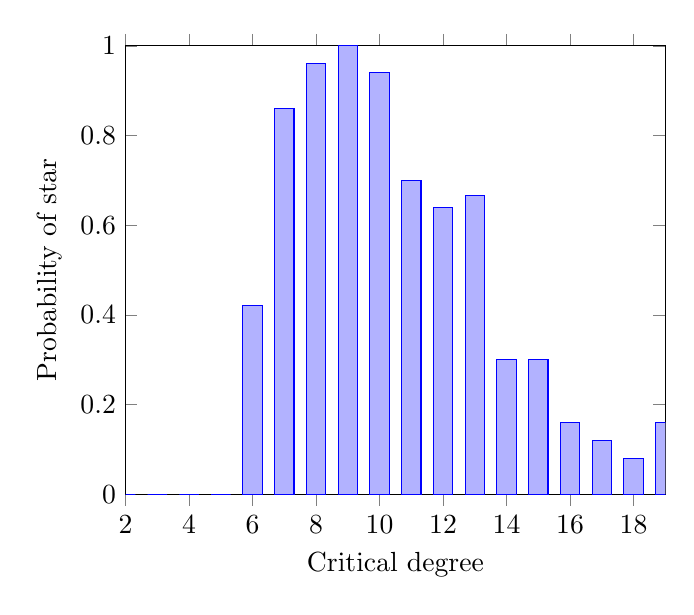
\begin{tikzpicture}
\begin{axis}[
x tick label style={
	/pgf/number format/1000 sep=},
	ylabel=Probability of star,
	xlabel=Critical degree,
enlargelimits=0.0,
legend style={at={(0.5,-0.15)},
anchor=north,legend columns=-1},
ybar,
bar width=7pt,
]
\addplot
coordinates {
(2,0.0) (3,0.0) (4,0.0) (5,0.0) (6,0.42) (7,0.86) 
(8,0.96) (9,1.0) (10,0.94) (11,0.70) (12,0.64)
 (13,0.667) (14,0.3) (15,0.3) 
(16,0.16) (17,0.12) (18,0.08) (19,0.16) };
\end{axis}
\end{tikzpicture}
\caption{\label{fig:PlotStar} Shows the probability of the network ending up in a star, given different critical degrees.}
\end{figure}

From Figure \ref{fig:PlotClique} we can observe that the opposite is happening when the critical degree is increased; the probability of the resulting network being a clique drastically decreases. As we can see with a critical degree of seven or higher, it is very unlikely that we end up with a clique. These findings support our conjectures.

\begin{figure}
\centering
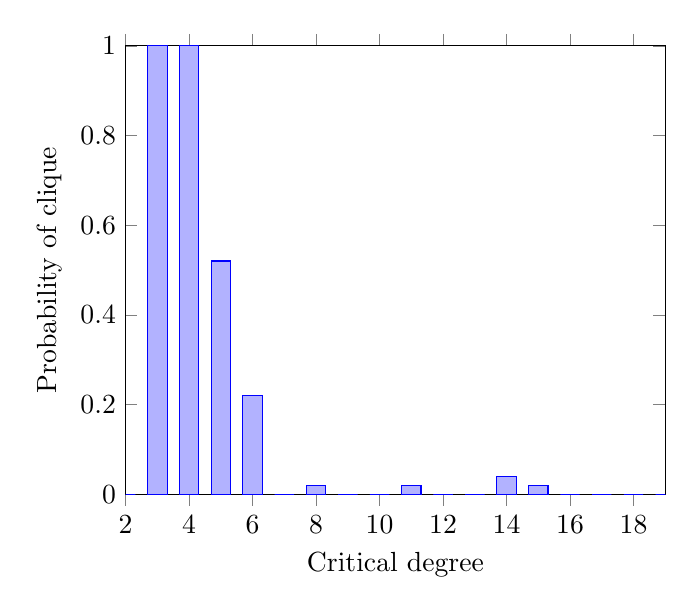
\begin{tikzpicture}
\begin{axis}[
x tick label style={
	/pgf/number format/1000 sep=},
	ylabel=Probability of clique,
	xlabel=Critical degree,
enlargelimits=0.0,
legend style={at={(0.5,-0.15)},
anchor=north,legend columns=-1},
ybar,
bar width=7pt,
]
\addplot
coordinates {
(2,0.0)(3,1.0) (4,1.0) (5,0.52) (6,0.22) (7,0.0) 
(8,0.02) (9,0.0) (10,0.00) (11,0.02) (12,0.0)
 (13,0.0) (14,0.04) (15,0.02) 
(16,0.0) (17,0.0) (18,0.00) (19,0.0) };
\end{axis}
\end{tikzpicture}
\caption{\label{fig:PlotClique} Shows the probability of the network ending up in a clique, given different critical degrees.}
\end{figure}

An interesting comparison can be made between the emergence of a star versus a clique. Figure \ref{fig:PlotStarVsClique} shows a plot of the network resulting in a star and another plot of the probability for the resulting network to become a clique. As we can see, from a critical degree of five to seven, the resulting network structure, changes from almost certainly ending up in a clique, to almost certainly ending up in a star structure. The reason is as mentioned before that when the critical degree is low, the likelihood of many nodes reaching the critical degree is high. And none of these would like to delete any links. Hence we end up with a clique. The reason why we end up with star structures is because it is less likely that many nodes end up reaching the critical degree, hence most of the nodes still prefer to rely on indirect links, but the ones that reach the critical degree prefer to connect to everyone. Since the nodes with critical degree, have high connectivity, nodes will prefer to be connected with these, compared with other nodes. Nodes prefer to be connected to the ones with critical degree, the nodes with critical degree would like to connect to everyone, and thus the structure evolves into a star, with the critical degree node in the center. 


\begin{figure}
\centering
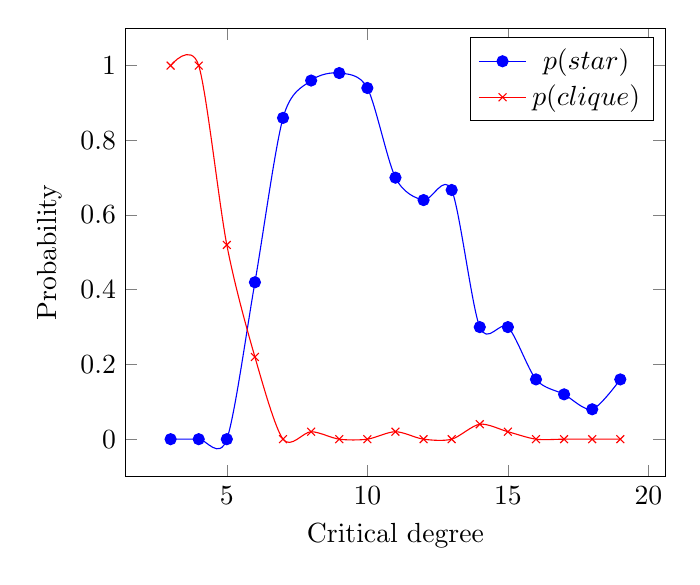
\begin{tikzpicture}
    \begin{axis}[
        xlabel=Critical degree,
        ylabel=Probability]
    \addplot[smooth,mark=*,blue] plot coordinates {
        (3,0.0) (4,0.0) (5,0.0) (6,0.42) (7,0.86) 
(8,0.96) (9,0.98) (10,0.94) (11,0.70) (12,0.64)
 (13,0.667) (14,0.3) (15,0.3) 
(16,0.16) (17,0.12) (18,0.08) (19,0.16)
    };
    \addlegendentry{$p(star)$}
    
    \addplot[smooth,color=red,mark=x]
        plot coordinates {
            (3,1.0) (4,1.0) (5,0.52) (6,0.22) (7,0.0) 
(8,0.02) (9,0.0) (10,0.00) (11,0.02) (12,0.0)
 (13,0.0) (14,0.04) (15,0.02) 
(16,0.0) (17,0.0) (18,0.00) (19,0.0)
        };
    \addlegendentry{$p(clique)$}
    \end{axis}
    \end{tikzpicture}
    \caption{\label{fig:PlotStarVsClique} Shows the comparison between the probability of the network ending up in a star (blue) or clique (red), given different critical degrees.}
\end{figure}

In Figure \ref{fig:PlotStar} when the critical degree gets closer to the number of nodes in the network, the probability of the network evolving into a star decreases. However, in Figure \ref{fig:PlotStarIsj}, we have plotted the probability of the network evolving into a network where only a few(2-4) nodes end up with a high degree, but not necessarily a critical degree. As we see, this occurs with high probability from critical degree six and up. These networks are so called scale-free networks (A-B graphs, described in the methodology chapter), because there are a few hubs, that account for most of the connectivity in the network. The reason why we end up with a scale-free network is because nodes prefer to be connected with nodes with high connectivity, and thus will delete links to nodes with low connectivity. This is very similar to the simple model that creates scale-free networks, where the probability of connecting to a node is proportional to the degree of the node.

\begin{figure}
\centering
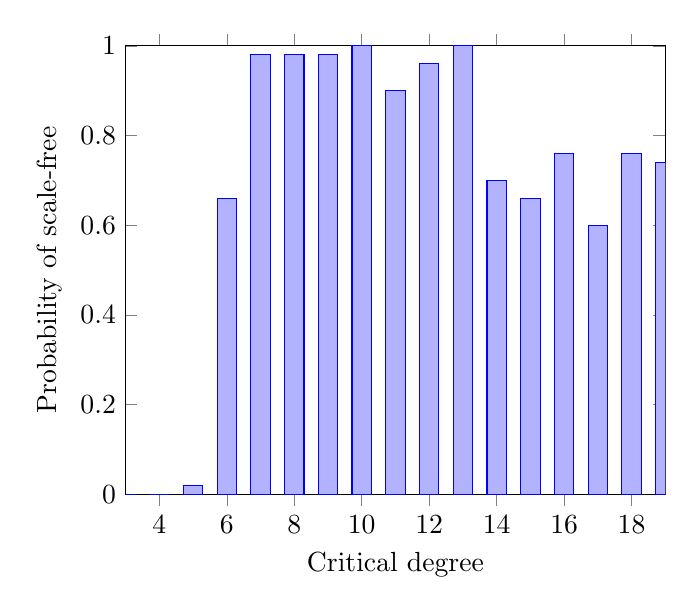
\begin{tikzpicture}
\begin{axis}[
x tick label style={
	/pgf/number format/1000 sep=},
	ylabel=Probability of scale-free,
	xlabel=Critical degree,
enlargelimits=0.0,
legend style={at={(0.5,-0.15)},
anchor=north,legend columns=-1},
ybar,
bar width=7pt,
]
\addplot
coordinates {
(3,0.0) (4,0.0) (5,0.02) (6,0.66) (7,0.98) 
(8,0.98) (9,0.98) (10,1.00) (11,0.90) (12,0.96)
 (13,1) (14,0.7) (15,0.66) 
(16,0.76) (17,0.60) (18,0.76) (19,0.74) };
\end{axis}
\end{tikzpicture}
\caption{\label{fig:PlotStarIsj} Shows the probability of the network ending up in a scale-free structure, given different critical degrees.}
\end{figure}
\paragraph{Price of Anarchy.}
Another interesting thing is the average price of anarchy as function of the critical degree. The price of anarchy was calculated by taking the average total payoffs and dividing on the optimal payoff. The result can be seen in Figure \ref{fig:plotpriceofanarchy}. 

We see that the price of anarchy for the first critical degrees is 1, and then decreases until degree six, and at seven it increases again. This is because at degree one to five, the socially optimal structure is a clique. At degree six, a clique and a star, are almost equally good, and at degree seven and up, a star structure is the socially optimal outcome. 
In other words, when the cost is low, a clique is the optimal structure, and when the cost is high a star is the optimal structure. 

This further improves our findings, because we have now shown how an insurer can determine the resulting network formation by changing the cost. In addition, the formation that evolves has a price of anarchy close to 1. 

\begin{figure}
\centering
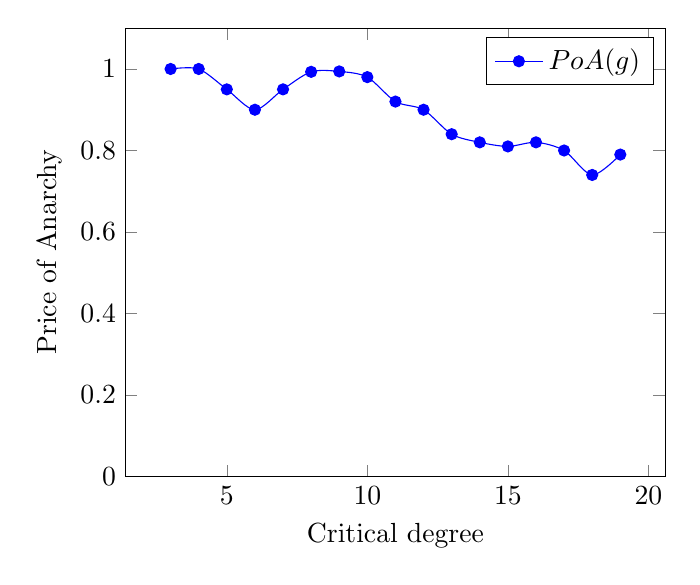
\begin{tikzpicture}
\begin{axis}[
	ylabel=Price of Anarchy,
	ymin=0.0,
	xlabel=Critical degree]
\addplot [smooth,mark=*,blue] plot coordinates {

(3,1) (4,1) (5,0.95) (6,0.9) (7,0.95) 
(8,0.993) (9,0.994) (10,0.98) (11,0.92) (12,0.90)
 (13,0.84) (14,0.82) (15,0.81) 
(16,0.82) (17,0.8) (18,0.74) (19,0.79) };
\addlegendentry{$PoA(g)$}
\end{axis}
\end{tikzpicture}
\caption{\label{fig:plotpriceofanarchy} Shows the price of anarchy as a function of critical degree}
\end{figure}

\paragraph{Example structures from the simulation.}


\begin{figure}
  \centering
  \includegraphics[width=0.7\linewidth]{../Figures/Clique-20-nodes.png}
  \caption{\label{fig:discountclique} A clique consisting of twenty nodes. }
\end{figure}

\begin{figure}
  \centering
  \includegraphics[width=0.7\linewidth]{../Figures/Clique-ish-20-nodes.png}
  \caption{\label{fig:discountbaloon} A network with high average node degree, but not a clique.}
\end{figure}
{\label{fig:discounthighdegree} Two different outcomes of the simulations where the critical degree is low}

In Figure \ref{fig:discounthighdegree} we see two of the many possible outcomes when the critical degree is achieved at a low node degree. As we see, most of the nodes have reached the critical degree, and thus connected to every other node.
In Figure \ref{fig:star1} we see one example of a scalefree network, and the standard star network, both with twenty nodes, and results from the simulations when the critical degree was set to a value above six. 

\begin{figure}
 \includegraphics[width=0.7\linewidth]{../Figures/Star-20-nodes.png}
  \caption{\label{fig:star:a} A star consisting of twenty nodes}
\end{figure}

  
\begin{figure}
  \centering
  \includegraphics[width=0.7\linewidth]{../Figures/Scalefree-20-nodes.png}
  \caption{\label{fig:star:b} A scalefree network with twenty nodes, where three nodes account for most of the connectivity.}
\end{figure}
{\label{fig:star1} Two different outcomes from running simulations with a high critical degree.}





\section{Discussion}
In this paper we have introduced tree different models of endogenous network formation. The first model can be applied to certain real-world scenarios, such as software development firms/chains, or other networks where the final product is dependent on the collaboration of multiple participants.
This was done by letting node get a bonus, which is first received when a node reaches the desired number of links (called max-degree). This made the separation process of insured and non-insured nodes difficult for the insurer. Due to the possibility of achieving the bonus, a node will have a high incentive to establish links, and is thus more accepting towards establishing links with risky nodes, compared to a scenario without bonus. The conditions for separating insured and non-insured nodes in this model are: $\beta+\gamma-r<I_{l}<\beta+\frac{\gamma}{m}$. For the separation of insured and non-insured nodes to be possible, the following has to hold: $1-\frac{1}{m}<\frac{r}{m}$. As we see, as $\gamma$ and/or $m$ increases, this gets more and more difficult to achieve. 

In Model 2 we tried to implement a common feature used by insurance companies, bulk discount, in order to see how this affected the network formation. The cost of insuring a link is now dependent on the node's degree. 
The discount resulted in higher incentive for insured nodes to establish links with non-insured nodes. The reason is intuitive, since the cost of doing so decreases as the node degree increases. 
The condition to ensure separation becomes: $m(\beta+\gamma-r)<I_{l}<\beta+\frac{\gamma}{m}$, it is now harder for the insurer to separate the insured and non-insured from eachother. 

To ensure separation the insurer has to set a higher price to compensate for the increased incentive of link establishment, therefore the potential price of anarchy is higher than in model 1.

In our last model we applied the discount to an already existing model, "the symmetric connection game". In this old game it has been shown that there are three different efficient and stable networks, clique, star and an empty network, that arise under certain cost conditions. If $I_{l}<\beta-\beta^{2}$, the efficient and stable network is a clique. If $\beta-\beta^{2}<I_{l}<\beta$ a star is both stable and efficient. If $I_{l}>\beta+\frac{N-2}{2}\beta^{2}$ an empty network is both stable and efficient. In general, a clique is the most efficient if the cost of establishing links is less than the benefit gained from indirect connections. A star is the most efficient if the cost is higher than the benefit from indirect connections, but less than the benefit of direct connections. 
However, it is proved that as the number of nodes in the networks increases, the probability of the network ending up in star goes to zero. But, when we applied our insurance discount to this model, we found conjectures saying that, by setting the cost to the right level, one can with high probability ensure that either a clique, a star or a scale-free structure will evolve. This changes the connection game drastically, because now the insurer is able to force the network into three possible network formations, where the star has a fixation probability that exceeds the cliques. The insurer can use these findings to ensure that one of the beneficial structures, star or clique evolves. If the insurer is able to force a star to evolve, this can be used to drastically increase the overall security, and at the same time minimize the overall link cost. 

\section{Conclusion}
From our background study, it was revealed that the current market for cyber-insurance is far from healthy, and many have failed in attempts to establish a cyber-insurance market.
As described in the introduction, there are certain obstacles that are unique for cyber-insurance, and arguably these are the reasons why cyber-insurance has not emerged as expected. 
 However, we believe that there is a need for cyber-insurance, and that our new approach of analyzing the cyber-insurance market through graphs and network formation games could help establishing and improving the market.

We studied a variety of different network formation games, in order to find out if there were any superior network topologies that would fit as a cyber-insurance network, were ideally both the insurer and customers get a higher payoff from purchasing cyber-insurance. 
We found that star and clique networks had appropriate characteristics, not only do they have calculable fixation probability, but they could also generate better security and overall higher payoff for the nodes. With these networks in mind, we wanted to find a way of forcing networks to evolve into these structures.  We found that insurers could adjust the insurance premium in order to control the formation of networks. If the price is set to the right level, networks with calculable risk will evolve, and if the insurer is able to separate the nodes into two different networks, one consisting of trusted, insured nodes, the other of non-insured nodes, the trusted nodes can even further increase their payoff, compared to a non-trusted network. The insurer now possesses a tool for setting the insurance premium properly, possible resulting in better products for both the customer and the insurer.

\paragraph{Limitations and future work}
One limitation to our work, and a suggestion for future work, is to map our models and simulations to real-world networks in a more convincing way. Real-world networks are not random. Nodes may prefer to talk to nodes with high degree or low degree. In addition, the decision to use additive risk were taken due to the simplicity of the function and the fact that we do not know how a real-world risk distribution actually looks like.  By introducing a complex risk function, we would only have distorted the goal of our models. i.e. suggestions for improving our models is to introduce more realistic payoff functions.
%
\begin{thebibliography}{[MT1]}
%
\bibitem[BO1]{bolot:cyber}
  Bolot, Jean and Lelarge, Marc:
  Cyber insurance as an incentive for Internet security
  Managing information risk and the economics of security
  (2008) 269--290
%
\bibitem[BO2]{bolot:cyber2}
	Lelarge, Mark, and Jean Bolot:
	Economic incentives to increase security in the internet: The case for insurance.
	INFOCOM (2009), IEEE.
%
\bibitem[BO3]{bolot:new}
	Bolot, Jean C and Lelarge, Marc
 	A new perspective on internet security using insurance
 	INFOCOM The 27th Conference on Computer Communications. IEEE
 	(2008) 1948--1956
  %
\bibitem[RA1]{ranjan:cyber}
	Pal, Ranjan and Hui, Pan	
	On Differentiating Cyber-Insurance Contracts A Topological Perspective
  	Internet Management Conference (2013), IEEE.
%
\bibitem[PO1]{ccost}
Ponemon Institute
Second Annual Cost of Cyber Crime Study, Benchmark Study of U.S: Companies
Ponemon Institute (2011)
%
\bibitem[ST1]{evolvingcyber}
  Evolving cyber cover
  \url{http://www.strategic-risk.eu/Journals/2012/02/22/i/j/w/RiskFinancing_Mar12.pdf}
  Accessed: 31/01/2013
  %
\bibitem[GN1]{CFCunder}
	Graeme Newman
	Cyber liability in Europe: What insurers should knowL
	CFC Underwriter \url{http://www.cfcunderwriting.com/media/news-articles/european-cyber.aspx}
 	Accessed: 14/02/2013
  %
  \bibitem[BS1]{bohme2010modeling}
  B{\"o}hme, R. and Schwartz, G.
  Modeling cyber-insurance: Towards a unifying framework
  Proceedings of GameSec (2010)
%
\bibitem[LE1]{lieberman2005evolutionary}
Lieberman, Erez and Hauert, Christoph and Nowak, Martin A
 Evolutionary dynamics on graphs
Nature Publishing Group 433-7023 (2005) 312--316
%
\bibitem[BL1]{contagion}
Blumen, L., Easley, D., Kleinber, J.,  Kleinberg, R. anad Tardon, E.
Network Formation in the Presence of Contagious Risk
MacArthur Foundation (2011)
 \bibitem[JM1]{jackson1996strategic}
 Jackson, Matthew O and Wolinsky, Asher
 A strategic model of social and economic networks
 New York: Academic Press Journal of economic theory 71-1 (1996) 44--74
%
\bibitem[JM2]{jackson2005survey}
Jackson, Matthew O
A survey of network formation models: Stability and efficiency
Group Formation in Economics: Networks, Clubs and Coalitions, ed. G. Demange and M. Wooders (2005) 11--57 

\end{thebibliography}
%

\end{document}
